%!TEX root = main.tex

\subsection{Semantics of {$\AOAMASS$} for the other versions of Android}

As mentioned before, the semantics of {$\AOAMASS$} of different versions of Android are different. In the sequel, we illustrate the differences by focusing on $\IFAOAMASS$. The differences of the semantics of {$\AOAMASS$} can be found in the appendix. 

Before a formal description, let us first illustrate the differences using the following example. 
\begin{example}
    Let $\Mm = (\act,A,\frag,\lmd,\aft,\vgr, \Delta)$ be an {$\IFAOAMASS$}, where $\act = \{A,B,C,D\}$, for each $A' \in\act$, $\lmd(A') = \STD$, $\aft(A) = \aft(B) = 1$, and $\aft(C) = \aft(D) = 2$, moreover, $\Delta = \{\back\} \cup  \{\tau_i \mid 1\le i \le 6\} \cup \{\tau'_i \mid 1\le i \le 3\} $ such that 
        $\tau_1 = A\xrightarrow{\startactivity(\bot)}C$,
        $\tau_2 = C\xrightarrow{\startactivity(\ntkflag\wedge\mtkflag)}B$,
        $\tau_3 = B\xrightarrow{\startactivity(\ntkflag)}C$,
        $\tau_4 = C\xrightarrow{\startactivity(\bot)}D$,
        $\tau_5 = D\xrightarrow{\startactivity(\bot)}A$,
        $\tau_6 = A\xrightarrow{\startactivity(\ntkflag)}A$,
        $\tau'_1 = C\xrightarrow{\startactivity(\ntkflag\wedge\rtfflag)}D$,
        $\tau'_2 = C\xrightarrow{\startactivity(\rtfflag)}A$,
        $\tau'_3 = C\xrightarrow{\startactivity(\ntkflag)}B$.

We use the configuration $(([CA],A,\mainflag),([ADC],C,\ntkflag),([B],B,\ntkflag))$ to illustrate the difference. This configuration can be reached from the initial configuration $(([A],A,\mainflag))$ by the following sequence of transition rules: $\tau_1\ \tau_2\ \tau_3\ \tau_4\ \tau_5\ \tau_6\ \back$.
%    As shown in Figure~\ref{and-example}, the configuration $((([CA],A,\mainflag),([ADC],C,\ntkflag),([B],B,\ntkflag)),\neg\nohflag)$ is reached from the initial configuration $((([A],A,\mainflag)),\neg\nohflag)$ by the transition rules sequence $\tau_1',\tau_2',\tau_3',\tau_4',\tau_5',\tau_6',\back$.
The differences of semantics for different versions of Android are demonstrated by applying $\tau'_1, \tau'_2, \tau'_3$ on the configuration $(([CA],A,\mainflag),([ADC],C,\ntkflag),([B],B,\ntkflag))$ (see Figure~\ref{fig-diff-version}).     
\begin{itemize}
 \item If the transition $\tau'_1 = C\xrightarrow{\startactivity(\ntkflag \wedge \rtfflag)}D$ is applied, then for Android 11.0-13.0 the task $([ADC],C,\ntkflag)$ is moved to the top and the activity $D$ is reordered to the front, resulting in the configuration
        $$(([DAC],C,\ntkflag), ([CA],A,\mainflag), ([B],B,\ntkflag)),$$ 
        while for Android 6.0-10.0,  the activity $D$ is pushed after the task $([ADC],C,\ntkflag)$ is moved to the top, resulting in the configuration 
        $$(([DADC],C,\ntkflag), ([CA],A,\mainflag), ([B],B,\ntkflag)).$$
        This difference is explained by the fact that for Android 6.0-10.0, $\rtfflag$ is ignored when it is used together with $\ntkflag$.
        
%        there is a distinction in the generated configurations between Android 6.0-10.0 and Android 11.0-12.0. In Android 6.0-10.0, $D$ is directly added to the $C$-task instead of being placed on top of the $C$-task. This implies that in Android 6.0-10.0, $\rtfflag$ becomes irrelevant to the semantics when it is combined with $\ntkflag$.
        %
        \item If the transition $\tau'_2 = C\xrightarrow{\startactivity(\rtfflag)} A$ is applied,  then for all the versions of Android 6.0--13.0, except 7.0, $A$ is reordered to the front in the top task, resulting in the configuration 
        $$(([AC],A,\mainflag),([ADC],C,\ntkflag),([B],B,\ntkflag)).$$
        In Android 7.0, the top task is cleared and $A$ is pushed, resulting in the configuration
        $$(([A],A,\mainflag),([ADC],C,\ntkflag),([B],B,\ntkflag)).$$
        This difference is explained by the fact that for Android 7.0, when the top task is the main task where the started activity occurs but is not the top activity, $\rtfflag$ has the same effect as $\ctkflag$.
                %
        \item If the transition $\tau'_3 = C\xrightarrow{\startactivity(\ntkflag)} B$ is applied, then for all the versions of Android 7.0--12.0,  the $B$-task is moved to the top (without pushing a new instance of $B$), resulting in the configuration 
        $$(([B],B,\ntkflag), ([CA],A,\mainflag),([ADC],C,\ntkflag)).$$
        In Android 6.0, the $B$-task is not moved to the top, and an instance of $B$ is pushed to the top task directly, resulting in the configuration
        $$(([BCA],A,\mainflag),([ADC],C,\ntkflag), ([B],B,\ntkflag)).$$
       This difference is explained by the fact that the task allocation mechanism of Android 6.0 is different from the other versions, namely, in Android 6.0, only affinities are used for looking for a task, while for the other versions, real activities and affinities are used together to look for a task. 
       %        the generated configuration of Android 6.0 is different with other versions. In Android 6.0, $B$-task is not switched to the top. This implies that the task allocation mechanism of Android 6.0 has nothing to do with the real activities of tasks but only uses the affinities of tasks.
        % that is, $\rtfflag$ is irrelevant to the semantics in this case.
    \end{itemize}

\begin{figure}[htbp]
    % \vspace{-3mm}
\centering
        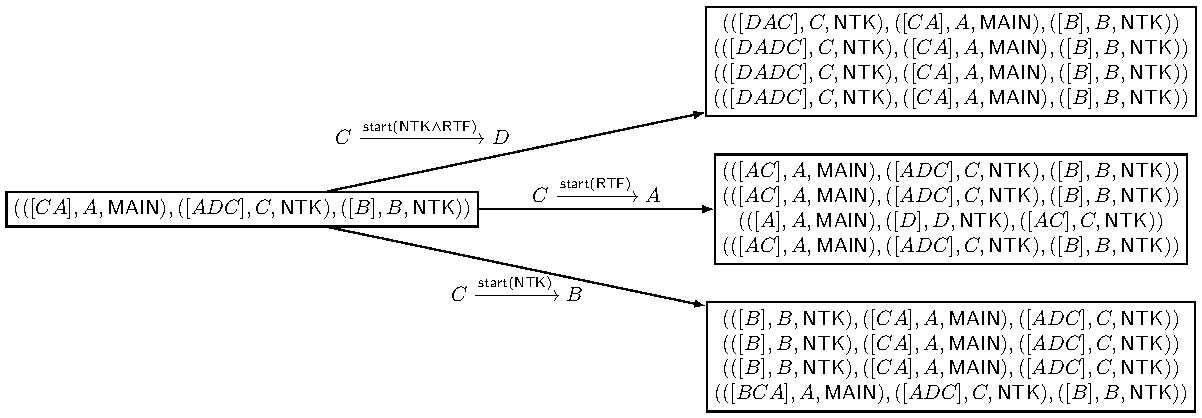
\includegraphics[scale = 0.7]{and-example.pdf}
\caption{Semantics of $\IFAOAMASS$ for different versions of Android, where the 1st, 2nd, 3rd, 4th line of the texts in the right boxes are configurations for Android 11.0--13.0, 8.0--10.0, 7.0, and 6.0 respectively}
    % \vspace{-6mm}	
    \label{fig-diff-version}
\end{figure}
\end{example}
%

In the sequel, we state the differences of the semantics of {$\IFAOAMASS$} models in details. To avoid tediousness, let us focus on the situation $\phi \models \neg \tohflag$. The differences for the situation $\phi \models \tohflag$ are similar. 

\subsubsection{Android 11.0, 12.0.}
The semantics of {\AMASS} for Android 11.0 and 12.0 are the same as Android 13.0. 

\subsubsection{Android 10.0, 9.0, and 8.0.}
The semantics for these three versions are the same and differ from that for Android 13.0 in the following sense: $\rtfflag$ is ignored when used together with $\ntkflag$. 
That is, for Android 10.0, 9.0, and 8.0, the semantics of $\IFAOAMASS$ for the case $\phi  \models \ntkflag \wedge \neg \ndmflag$ is adapted from Android 13.0 as follows.

\begin{itemize}
\item If $\phi \models \mtkflag$, then $\cdots$.
%
\item If $\phi \models \neg \mtkflag$, then
	\begin{itemize}
        \item if $\getrealtsk(\rho, B) = S_i$ or $\getrealtsk(\rho,B) = * \wedge\gettsk(\rho,B) = S_i$, then
		\begin{itemize}
			\item if $\phi \models \ctkflag$, then $\cdots$,
			\item if $\phi \models \neg \ctkflag$, then
			\begin{itemize}
				\item if $\phi \models \ctpflag$ and $B \in S_i$, then $\cdots$,
				\item if $\phi \models \ctpflag$ and $B \notin S_i$, then $\cdots$,
				\item if $\phi \models \neg \ctpflag$, then
				\begin{itemize}
						\item if $\getrealtsk(\rho, B) = S_i$ and $\zeta_i \neq \mainflag$, 
						then $\rho' = \mvtsktop(\rho, i)$,
						\item otherwise, 
						\begin{itemize}
							\item if $\phi \models \stpflag$ and $\topact(S_i) = B$, or $\phi \models \stpflag \wedge \pitflag$ and $i = 1$ and $\preact(S_1) = B$, then $\rho' = \mvtsktop(\rho, i)$,
							\item otherwise, $\rho'=\push(\mvtsktop(\rho, i), B)$,
						\end{itemize}
				\end{itemize}
			\end{itemize}
		\end{itemize}
	    %
	\item if $\gettsk(\rho, B) = *$, then $\cdots$.
	\end{itemize}
\end{itemize}
%When $\phi \models \ntkflag \wedge \neg\ndmflag\wedge\neg \mtkflag$, $\rtfflag$ is ignored. 
%
\hide{
\begin{itemize}
\item If $\phi \models \mtkflag$, then $\cdots$. 
\item If $\phi \models \neg \mtkflag$, then 
\begin{itemize}
    \item if $\getrealtsk(\rho, B) = S_i$ or $\getrealtsk(\rho,B) = * \wedge\gettsk(\rho,B) = S_i$, then
    \begin{itemize}
    \item if $i \neq 1$, then 
        \begin{itemize}
            \item if $\phi \models \ctkflag$, then $\cdots$ 
            \item if $\phi \models \neg \ctkflag$, then $\cdots$
                \begin{itemize}
                    \item if $\phi \models\ctpflag$ and $B \in S_i$, then $\cdots$
                    \item if $\phi \models\ctpflag$ and $B \notin S_i$, then $\cdots$
                    \item if $\phi \models\neg\ctpflag$, then
                    \begin{itemize}
                            \item if $\getrealtsk(\rho,B) = S_i$ and $\zeta_i \neq \mainflag$, then $b' = \neg \nohflag$, moreover,
                            \begin{itemize}
                                \item if $b = \neg \nohflag$, then $\rho'=\mvtsktop(\rho, i)$,
                                \item otherwise, $\rho' = \rmact(\mvtsktop(\rho, i), 2, 1)$, 
                            \end{itemize}
                            \item otherwise ($\getrealtsk(\rho,B) = S_i$ and $\zeta_i = \mainflag$ or $\getrealtsk(\rho,B) = * \wedge\gettsk(\rho,B) = S_i$), 
                            \begin{itemize}
                                \item if $\phi\models\stpflag$ and $\topact(S_i) = B$, then $b' = \neg \nohflag$, moreover,
                                \begin{itemize}
                                    \item if $b = \neg \nohflag$, then $\rho'=\mvtsktop(\rho, i)$,
                                    \item otherwise, $\rho' = \rmact(\mvtsktop(\rho, i), 2, 1)$, 
                                \end{itemize}
                                \item otherwise, $b' = \nohflag$ iff $\phi \models \nohflag$, moreover, 
                                \begin{itemize}
                                    \item if $b = \neg \nohflag$, then $\rho'=\push(\mvtsktop(\rho, i), B)$,
                                    \item otherwise, $\rho' = \rmact(\push(\mvtsktop(\rho, i), B), 2, 1)$, 
                                \end{itemize}
                        \end{itemize}
                    \end{itemize}
                \end{itemize}
        \end{itemize}
    \item otherwise ($i  = 1$),  
    \begin{itemize}
        \item if $\phi \models \ctkflag$, then $\cdots$, 
        \item if $\phi \models \neg \ctkflag$, then 
        \begin{itemize}
            \item if $\phi \models \ctpflag$ and $B \in S_1$, then $\cdots$
%				\begin{itemize}
%					\item if $\phi\models \neg \stpflag$, then $b' = \nohflag$ iff $\phi \models \nohflag$, 
%					\item otherwise, $b' = \neg \nohflag$,
%				\end{itemize}
            \item if $\phi \models \ctpflag$ and $B\notin S_1$, then $\cdots$
            \item if $\phi \models \neg \ctpflag$, then
            \begin{itemize}
                \item if $\getrealtsk(\rho,B) = S_1$ and $\zeta_1 \neq \mainflag$, then $\rho' = \rho$ and $b' = b$,
                \item otherwise ($\getrealtsk(\rho,B) = S_1$ and $\zeta_i = \mainflag$ or $\getrealtsk(\rho,B) = * \wedge\gettsk(\rho,B) = S_1$), 
                \begin{itemize}
                    \item if $\phi\models\stpflag$ and $A = B$, or $\phi \models\stpflag\wedge\pitflag$ and $\preact(\rho) = B$, then $\rho' = \rho$ and $b' = b$, 
                    \item otherwise, $b' = \nohflag$ iff $\phi \models \nohflag$, moreover, 
                    \begin{itemize}
                        \item if $b = \neg \nohflag$, then $\rho'=\push(\rho, B)$,
                        \item otherwise, $\rho' = \rmact(\push(\rho, B), 1, 2)$, 
                    \end{itemize}
                \end{itemize}
            \end{itemize}
        \end{itemize}
    \end{itemize}
\end{itemize}
\item if $\gettsk(\rho, B) = *$, then $\cdots$. 
\end{itemize}
\end{itemize}
}
Note that the parts of the semantics denoted by $\cdots$ are the same as Android 13.0, and in the semantics for the situation $\phi \models \neg \ctpflag$, the flag $\rtfflag$ has no effects, thus is ignored.  


%Moreover, the semantics in the case $\phi \models \tohflag$ should be similarly adapted for $\rtfflag$.

%$\rtfflag$ flag will be omitted when $\phi\models\ntkflag$ or $\lmd(A) = \singleinstance$ for $A\xrightarrow{\alpha(\phi)}B$. More precisely, the semantics can be adapted from that for Android 12.0 as follows:
%\begin{itemize}
%    \item for the subcase $\phi \models \ntkflag\wedge \neg \mtkflag$, or $\lmd(A) = \singleinstance$ and $\phi  \models \neg \mtkflag$ of the case $\lmd(B) = \standard$ and $\lmd(B) = \singletop$, 
 %       remove $\rtfflag$ in the formulae $\phi$, and remove the item which constraint is $\phi\models\rtfflag\wedge\neg\ctpflag\wedge\neg\ctkflag$ and $B\in S_j$.
%\end{itemize}

\subsubsection{Android 7.0.}
The semantics for Android 7.0 is close to that of Android 10.0 (or 9.0, 8.0) but differs from it in the following two aspects:  1) the effect of $\ndmflag$ is the same as that of $\ntkflag$, 2)
when $\phi \models \neg \ntkflag \wedge \neg\ndmflag \wedge \neg\ctpflag$, if the top task is the main task where the started activity occurs but is not the top activity, then $\rtfflag$ has the same effect as $\ctkflag$. More precisely, for Android 7.0, only two cases $\phi \models \ntkflag$ and $\phi  \models \neg \ntkflag$ are considered, where the semantics for the case $\phi \models \ntkflag$ inherits that of $\phi \models \ntkflag \wedge \neg \ndmflag$ for Android 10.0, while the semantics for the case $\phi  \models \neg \ntkflag$ is adapted from that of $\phi \models \neg \ntkflag \wedge \neg \ndmflag$ for Android 10.0 as follows. 
%
%
%        \item if $\phi \models \rtfflag \wedge \neg \ctpflag$ and $B \in \toptsk(\rho)$, then
 %        $\rho'=\mvacttop(\rho, B)$,
%
\begin{itemize}
	\item If $\phi \models \ctpflag$ and $B \in \toptsk(\rho)$, then $\cdots$.
	\item If $\phi \models \ctpflag$ and $B \not \in \toptsk(\rho)$, then $\cdots$.
	\item If $\phi \models \neg \ctpflag$, then
		\begin{itemize}
    			\item if $\phi \models \rtfflag$ and $B \in \toptsk(\rho)$, then
    			\begin{itemize}
                    \item if $\zeta_i = \mainflag$, then $\rho' = \clrtsk(\rho, B)$,
                    \item otherwise, $\rho' = \mvacttop(\rho, B)$,
                    % \begin{itemize}
                    %         \item if $b = \neg \nohflag$, then $\rho'= \mvacttop(\rho, B)$, 
                    %         \item otherwise, $\rho' = \rmact(\mvacttop(\rho, B), 1, 2)$, 
                    % \end{itemize}
    			\end{itemize}
			\item if $\phi \models \rtfflag$ and $B \not \in \toptsk(\rho)$, then $\cdots$,
			\item if $\phi \models \neg \rtfflag$, then $\cdots$.
		\end{itemize}
\end{itemize}
%Intuitively, when $\phi \models \rtfflag \wedge \neg \ctpflag$, $B \in \toptsk(\rho)$, and additionally the top task is the main task, the top task is cleared before pushing $B$.

%$\ndmflag$ has the same effects with $\ntkflag$, and for each item $\ndmflag$ and $\neg\ndmflag$ are removed.

%In Android 7.0, $\rtfflag$ flag will clear the task when the current task is the main task. More precisely, the semantics of Android 7.0 is defined as follows.
%\begin{itemize}
%    \item for the subcase $\lmd(A) \neq \singleinstance$ and $\phi \models \neg \ntkflag$ of the case $\lmd(B) = \standard$ and $\lmd(B) = \singletop$, replace the constraint with $\phi\models\rtfflag\wedge\neg\ctpflag$ and $B\in S_j$ and $b_1=0$,
%        of the item which constraint is $\phi\models\rtfflag\wedge\neg\ctpflag$ and $B\in S_j$,
%        and add an item: if $\phi\models\rtfflag\wedge\neg\ctpflag$ and $B\in S_j$ and $b_1=1$,
%        then $\rho' = \push(\clrtsk(\rho),B)$.
%\end{itemize}

\subsubsection{Android 6.0.}
The semantics for Android 6.0 differs from that of Android 10.0 (or 9.0, 8.0) in the following two aspects: 1) the effect of $\ndmflag$ is the same as that of $\ntkflag$, 2) the task allocation mechanism of Android 6.0 does not use the real activities of tasks and only relies on affinities. 
%
More precisely, for Android 6.0, only two cases $\phi \models \ntkflag$ and $\phi  \models \neg \ntkflag$ are considered, where
the semantics for the case $\phi  \models \neg \ntkflag$ inherits that of $\phi \models \neg \ntkflag \wedge \neg \ndmflag$, 
and the semantics for the case $\phi \models \ntkflag$ is adapted from that of $\phi \models \ntkflag \wedge \neg \ndmflag$ for Android 10.0 as follows, where the conditions involving $\getrealtsk(\rho, B)$ and $\gettsk(\rho, B)$ are simplified into the conditions involving only $\gettsk(\rho, B)$, moreover, we do not need to distinguish whether a task is the main task or not.  
\begin{itemize}
\item If $\phi \models \mtkflag$, then $\cdots$.
%
\item If $\phi \models \neg \mtkflag$, then
	\begin{itemize}
        \item if $\gettsk(\rho,B) = S_i$, then
		\begin{itemize}
			\item if $\phi \models \ctkflag$, then $\cdots$,
			\item if $\phi \models \neg \ctkflag$, then
			\begin{itemize}
				\item if $\phi \models \ctpflag$ and $B \in S_i$, then $\cdots$,
				\item if $\phi \models \ctpflag$ and $B \notin S_i$, then $\cdots$,
				\item if $\phi \models \neg \ctpflag$, then
				\begin{itemize}
                    \item if $\phi \models \stpflag$ and $\topact(S_i) = B$, or $\phi \models \stpflag \wedge \pitflag$ and $i = 1$ and $\preact(S_1) = B$, then $\rho' = \mvtsktop(\rho, i)$,
                    \item otherwise, $\rho'=\push(\mvtsktop(\rho, i), B)$,
				\end{itemize}
			\end{itemize}
		\end{itemize}
	    %
	\item if $\gettsk(\rho, B) = *$, then $\cdots$.
	\end{itemize}
\end{itemize}
\hide{
\begin{itemize}
\item If $\phi \models \mtkflag$, then $\cdots$.
\item If $\phi \models \neg \mtkflag$, then 
\begin{itemize}
    \item if $\gettsk(\rho,B) = S_i$, then
%    // {\it $\getrealtsk(\rho, B) = S_i$ or $\getrealtsk(\rho,B) = * \wedge\gettsk(\rho,B) = S_i$ is replaced by $\gettsk(\rho,B) = S_i$}
    \begin{itemize}
    \item if $i \neq 1$, then 
        \begin{itemize}
            \item if $\phi \models \ctkflag$, then $\cdots$ 
            \item if $\phi \models \neg \ctkflag$, then $\cdots$
                \begin{itemize}
                    \item if $\phi \models\ctpflag$ and $B \in S_i$, then $\cdots$
                    \item if $\phi \models\ctpflag$ and $B \notin S_i$, then $\cdots$
                    \item if $\phi \models\neg\ctpflag$, then
%                    \begin{itemize}
%                            \item if $\getrealtsk(\rho,B) = S_i$ and $\zeta_i \neq \mainflag$, then $b' = \neg \nohflag$, moreover,
%                            \begin{itemize}
%                                \item if $b = \neg \nohflag$, then $\rho'=\mvtsktop(\rho, i)$,
%                                \item otherwise, $\rho' = \rmact(\mvtsktop(\rho, i), 2, 1)$, 
%                            \end{itemize}
%                            \item otherwise ($\getrealtsk(\rho,B) = S_i$ and $\zeta_i = \mainflag$ or $\getrealtsk(\rho,B) = * \wedge\gettsk(\rho,B) = S_i$), 
                            \begin{itemize}
                                \item if $\phi\models\stpflag$ and $\topact(S_i) = B$, then $b' = \neg \nohflag$, moreover,
                                \begin{itemize}
                                    \item if $b = \neg \nohflag$, then $\rho'=\mvtsktop(\rho, i)$,
                                    \item otherwise, $\rho' = \rmact(\mvtsktop(\rho, i), 2, 1)$, 
                                \end{itemize}
                                \item otherwise, $b' = \nohflag$ iff $\phi \models \nohflag$, moreover, 
                                \begin{itemize}
                                    \item if $b = \neg \nohflag$, then $\rho'=\push(\mvtsktop(\rho, i), B)$,
                                    \item otherwise, $\rho' = \rmact(\push(\mvtsktop(\rho, i), B), 2, 1)$, 
                                \end{itemize}
                           \end{itemize}
%                    \end{itemize}
                \end{itemize}
        \end{itemize}
    \item otherwise ($i  = 1$),  
    \begin{itemize}
        \item if $\phi \models \ctkflag$, then $\cdots$, 
        \item if $\phi \models \neg \ctkflag$, then 
        \begin{itemize}
            \item if $\phi \models \ctpflag$ and $B \in S_1$, then $\cdots$
%				\begin{itemize}
%					\item if $\phi\models \neg \stpflag$, then $b' = \nohflag$ iff $\phi \models \nohflag$, 
%					\item otherwise, $b' = \neg \nohflag$,
%				\end{itemize}
            \item if $\phi \models \ctpflag$ and $B\notin S_1$, then $\cdots$
            \item if $\phi \models \neg \ctpflag$, then
%            \begin{itemize}
%                \item if $\getrealtsk(\rho,B) = S_1$ and $\zeta_1 \neq \mainflag$, then $\rho' = \rho$ and $b' = b$,
%                \item otherwise ($\getrealtsk(\rho,B) = S_1$ and $\zeta_i = \mainflag$ or $\getrealtsk(\rho,B) = * \wedge\gettsk(\rho,B) = S_1$), 
                \begin{itemize}
                    \item if $\phi\models\stpflag$ and $A = B$, or $\phi \models\stpflag\wedge\pitflag$ and $\preact(\rho) = B$, then $\rho' = \rho$ and $b' = b$, 
                    \item otherwise, $b' = \nohflag$ iff $\phi \models \nohflag$, moreover, 
                    \begin{itemize}
                        \item if $b = \neg \nohflag$, then $\rho'=\push(\rho, B)$,
                        \item otherwise, $\rho' = \rmact(\push(\rho, B), 1, 2)$, 
                    \end{itemize}
%                \end{itemize}
            \end{itemize}
        \end{itemize}
    \end{itemize}
\end{itemize}
\item if $\gettsk(\rho, B) = *$, then $\cdots$. 
\end{itemize}
\end{itemize}
}
%remove the item and sub-items for the constraint $\getrealtsk(\rho, B) = S_i$ and $\zeta_i \neq \mainflag$, and replace  the following constraint with  $ \gettsk(\rho, B) = S_i$: $\getrealtsk(\rho, B) = S_i$ and $\zeta_i = \mainflag$, or $\getrealtsk(\rho, B) = * \wedge \gettsk(\rho, B) = S_i$.
	%
%	remove the item corresponding to the constraint $\getrealtsk(\rho, B) = S_j$, moreover, replace the constraint $\getrealtsk(\rho, B) = *$ and $\gettsk(\rho, B) = S_j$ with $\gettsk(\rho, B) = S_j$.
	%
%
We remark that the unexpected behavior of $\rtfflag$ for Android 7.0, that is, $\rtfflag$ behaves the same as $\ctkflag$ in some cases, does not occur in Android 6.0. 
